
    \begin{figure}[H]
      {
        \setlength{\tabcolsep}{3.0pt}
        \setlength\cmidrulewidth{\lightrulewidth} % Make cmidrule = 
        \begin{adjustbox}{width=0.8cm,center}
          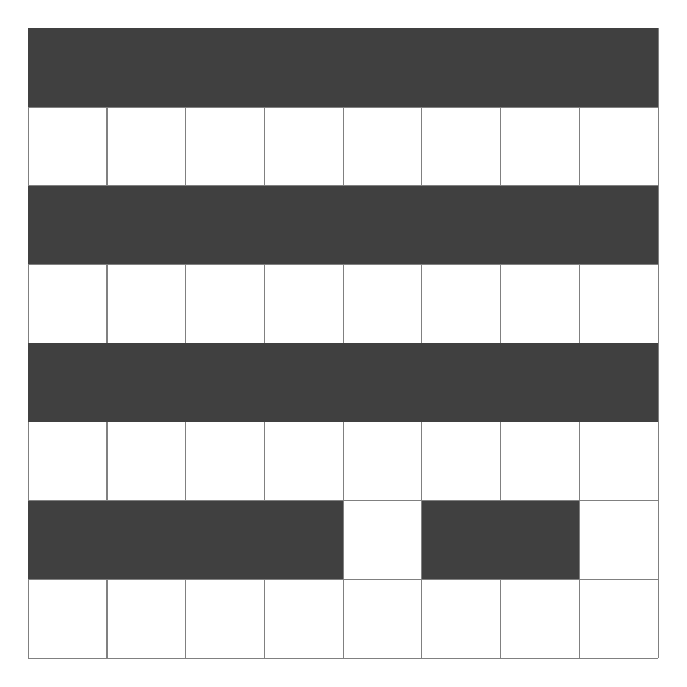
\begin{tikzpicture}
    
\def\CHARCOLOR{darkgray}
	\draw[step=1.0,gray,thin] (0,0) grid (8,8);
	\fill[\CHARCOLOR] (0,7) rectangle ++ (1,1);
	\fill[\CHARCOLOR] (1,7) rectangle ++ (1,1);
	\fill[\CHARCOLOR] (2,7) rectangle ++ (1,1);
	\fill[\CHARCOLOR] (3,7) rectangle ++ (1,1);
	\fill[\CHARCOLOR] (4,7) rectangle ++ (1,1);
	\fill[\CHARCOLOR] (5,7) rectangle ++ (1,1);
	\fill[\CHARCOLOR] (6,7) rectangle ++ (1,1);
	\fill[\CHARCOLOR] (7,7) rectangle ++ (1,1);
	\fill[\CHARCOLOR] (0,5) rectangle ++ (1,1);
	\fill[\CHARCOLOR] (1,5) rectangle ++ (1,1);
	\fill[\CHARCOLOR] (2,5) rectangle ++ (1,1);
	\fill[\CHARCOLOR] (3,5) rectangle ++ (1,1);
	\fill[\CHARCOLOR] (4,5) rectangle ++ (1,1);
	\fill[\CHARCOLOR] (5,5) rectangle ++ (1,1);
	\fill[\CHARCOLOR] (6,5) rectangle ++ (1,1);
	\fill[\CHARCOLOR] (7,5) rectangle ++ (1,1);
	\fill[\CHARCOLOR] (0,3) rectangle ++ (1,1);
	\fill[\CHARCOLOR] (1,3) rectangle ++ (1,1);
	\fill[\CHARCOLOR] (2,3) rectangle ++ (1,1);
	\fill[\CHARCOLOR] (3,3) rectangle ++ (1,1);
	\fill[\CHARCOLOR] (4,3) rectangle ++ (1,1);
	\fill[\CHARCOLOR] (5,3) rectangle ++ (1,1);
	\fill[\CHARCOLOR] (6,3) rectangle ++ (1,1);
	\fill[\CHARCOLOR] (7,3) rectangle ++ (1,1);
	\fill[\CHARCOLOR] (0,1) rectangle ++ (1,1);
	\fill[\CHARCOLOR] (1,1) rectangle ++ (1,1);
	\fill[\CHARCOLOR] (2,1) rectangle ++ (1,1);
	\fill[\CHARCOLOR] (3,1) rectangle ++ (1,1);
	\fill[\CHARCOLOR] (5,1) rectangle ++ (1,1);
	\fill[\CHARCOLOR] (6,1) rectangle ++ (1,1);

          \end{tikzpicture}
        \end{adjustbox}
      }\caption*{\$BF}
    \end{figure}
    